\documentclass[16pt, a4paper]{article}
\usepackage[utf8]{inputenc}
\usepackage{fancyhdr}
\usepackage{graphicx}
\usepackage[left=3cm,right=3cm,top=3cm,bottom=3cm]{geometry}
\graphicspath{ {./images/} }

\usepackage[document]{ragged2e}
\usepackage{amsmath}
\justifying

\rfoot{\thepage}

\title{Projet MOGPL}
\date{2022}
\begin{document}

\begin{center}
    \vspace*{\fill}
    \textbf {
        \vspace*{10mm}
        \Large {Projet MOGPL \\}
        \vspace*{7mm}
        \noindent\rule[0.25\baselineskip]{\textwidth}{1pt}\\
        \vspace*{7mm}
        \LARGE{Optimisation Equitable\\}
        \vspace*{7mm}
        \noindent\rule[0.25\baselineskip]{\textwidth}{1pt}\\
        \vspace*{50mm}
        \Large {Fanxiang Zeng \\Zhe Wang\\} 
        \vspace*{20mm}
   }
    
       
        \vspace*{30mm}
   
        	\begin{center}
    		\begin{figure*}[!ht]
    			\centering{
\includegraphics[scale=0.4]{imgs/sorbonnelogo.png}}
    	    \end{figure*}
    	\end{center}
    \vspace*{\fill}
    %\vspace*{10mm}
        %\Large {Faculté des Sciences\\Sorbonne Univesité 2021-2022}
        \large {15 Mars 2022}
    \end{center}



\begin{flushleft}
\newpage

\pagestyle{fancy}

\fancyhf{}  
\rfoot{\thepage}
\rhead{}
\rhead{Projet MOGPL : optimisation équitable}
\setcounter{tocdepth}{1}
\tableofcontents
\newpage
\begin{justify}

\section{Linéarisation de \begin{math}f\end{math}}
\setlength{\parindent}{0ex}
\subsection{}
\large{
soit 
$$ \min \sum_{i=1}^{n} a_{ik}z_i $$
$$ s.c. \sum_{i=1}^{n} a_{ik} = k $$
$$ a_{ik}\in{\{0,1\}}, i = 1,...,n $$
qui cherche a minimiser le somme des $ a_{ik}z_i $ avec $ a_{ik}\in{\{0,1\}} $ et comme contrainte $\sum_{i=1}^{n} a_{ik} = k $. Du coup, nous avons au strictement $k z_i$ pour satisfaire la contrainte. Pour minimiser $ \sum_{i=1}^{n} a_{ik}z_i $, on doit choisir les plus petits $z_i$ et comme $ z_i $ est strictement croissant, les plus petits $z_i$ sont les i-premiers$ z_i$ ce qui correspondrait du coup à $\sum_{i=1}^k z(i) $ et nous avons

$$ L_K (z)  = \sum_{i=1}^k z(i) $$
Donc $L_k$ est équivalent au minimum de notre fonction objectif, qui représente l'optimalité de $ \min \sum_{i=1}^{n} a_{ik}z_i $

}


\subsection{}

soit P : 
$$
\min \sum_{i=0}^n a_{ik} z_i 
$$
\begin{center}
\begin{math}
\begin{cases}
    \sum_{i=1}^n a_{ik}=k \\
    a_{ik} \leq 1 \\
\end{cases}
\end{math}
\end{center}
$$
 a_{ik} \geq 0 , i = 1, \cdots , n
$$


le dual D de P  
$$ \max kr_{k} - \sum_{i=0}^n b_{ik}$$
$$ s.c. \left\{ r_k - b_{ik} \leq z_i \right.$$
$$b_{ik} \geq 0, i=1, \cdots, n$$


Calculons par programmation lineaire les composantes du vecteur L(4, 7, 1, 3, 9, 2) 
$$ \max kr_{k} - \sum_{i=0}^6 b_{ik}$$
\begin{center}
\begin{math}
s.c. \begin{cases}
    r_k - b_{1k} \leq 1\\
    r_k - b_{2k} \leq 2\\
    r_k - b_{3k} \leq 3\\
    r_k - b_{4k} \leq 4\\
    r_k - b_{5k} \leq 7\\
    r_k - b_{ik} \leq 9\\
\end{cases}
\end{math}
\end{center}
nous obtenons tel programmation lineaire avec $z_i$ strictement croissant.
en mettant ce PL dans gurobi solver nous trouvons : 
$$ L_1(z) =1  , L_2(z) =3 , L_3(z) = 6 , L_4(z) = 10 , L_5(z) = 17 , L_6(z) = 26 $$ 

\subsection{}

\begin{align*}
& \ \ \ \ \sum_{k=1}^n w'_kL_k(z(x))\\
& =\sum_{k=1}^{n-1} w'_kL_k(z(x))+w'_nL_n(z(x))\\
& =\sum_{k=1}^{n-1}(w_k-w_{k+1})\sum_{i=1}^kz_i(x)+w_n\sum_{i=1}^nz_i(x)\\
& =\sum_{k=1}^{n-1}w_k\sum_{i=1}^kz_i(x)-\sum_{k=1}^{n-1}w_{k+1}\sum_{i=1}^kz_i(x)+w_n\sum_{i=1}^nz_i(x)\\
& =w_1z_1+w_2(z_1+z_2)+w_3(z_1+z_2+z_3)+...+w_{n-1}(z_1+...+z_{n-1})+w_n(z_1+...+z_n)\\
& \ \ \ \ -(w_2(z_1)+w_3(z_1+z_2)+...+w_n(z_1+...+z_{n-1}))\\
& =w_1z_1+w_2z_2+...+w_nz_n\\
& =\sum_{i=1}^nw_iz_i\\
& =f(x)
\end{align*}

\subsection{}
La maximisation de f(x) sur un ensemble X decrit par des contraintes lineaire peut s’ecrire sous la forme du programme lineaire suivant:

$$\max \sum_{k=1}^n w'_k(kr_k- \sum_{i=1}^n b_{ik})$$
\begin{center}
\begin{math}
s.c. \begin{cases}
    r_k - b_{ik} \leq z_i(x) , i = 1,\cdots,n\\
    x \in X
    \end{cases}
\end{math}
\end{center}
$$b_{ik} \geq 0 , i = 1,\cdots,n\\$$

Reformulons le probleme de l'exemple 1 avec cette linearisation


\begin{align*}
&\max \sum_{k=1}^2 w'_k(kr_k- \sum_{i=1}^2 b_{ik})\\
& = w'_1(r_1- \sum_{i=1}^2 b_{i1}) + w'_2(2r_2- \sum_{i=1}^2 b_{i2})\\
\end{align*}
\begin{math}
s.c. \begin{cases}
    r_k - b_{ik} \leq z_i(x)\\
    x \in X
\end{cases} 
\iff
s.c. \begin{cases}
    r_1 - b_{11} \leq z_1(x) = 5x_1 + 6x_2 + 4x_3 + 8x_4 +x_5 \\
    r_1 - b_{12} \leq z_1(x) = 5x_1 + 6x_2 + 4x_3 + 8x_4 +x_5  \\
    r_2 - b_{21} \leq z_2(x) = 3x_1 + 8x_2 + 6x_3 + 2x_4 + 5x_5 \\
    r_2 - b_{22} \leq z_2(x) = 3x_1 + 8x_2 + 6x_3 + 2x_4 + 5x_5 \\
    x1 + x2 + x3 +x4 + x5 = 3
\end{cases}\\
\end{math}
$$r_{k}, b_{ik} \geq 0 ; i,k\in \{1,2\} ; x_i \in \{0,1\}\\$$

Remarque : ici les $w'_k$ sont des poids qui sont fixees par les utilisateurs nous pourront les fixees a 1 pour le moment pour les enlever de la fonction objectif. 

reecrivons le PL en mettant tous les variables a gauches : 

\begin{align*}
\max r_1- \sum_{k=1}^2 b_{i1} + 2r_2- \sum_{i=1}^2 b_{i2}
\end{align*}
\begin{center}
    \begin{math}
        s.c.\begin{cases}
        r_1 - b_{11} - 5x_1 - 6x_2 - 4x_3 - 8x_4 - x_5    \leq 0  \\
        r_1 - b_{12} - 5x_1 - 6x_2 - 4x_3 - 8x_4 - x_5   \leq 0 \\
        r_2 - b_{21} - 3x_1 - 8x_2 - 6x_3 - 2x_4 - 5x_5 \leq 0 \\
        r_2 - b_{22}  - 3x_1 - 8x_2 - 6x_3 - 2x_4 - 5x_5  \leq 0 \\
        x1 + x2 + x3 +x4 + x5 = 3
        \end{cases}\\
    \end{math}
\end{center}
$$r_{k}, b_{ik} \geq 0 ; i,k\in \{1,2\} ; x_i \in \{0,1\}\\$$

En entrant le PL dans le gurobi solver nous trouvons comme resultat : 
$$ x_1 = 0 ; x_2 = 1 ; x_3 = 1 ; x_4 = 0 ; x_5 = 0$$
$$ r_1 = 16, r_2 = 18$$
$$ b_{11} = 0  , b_{12} =0 ,b_{21} =0 , b_{22} =2 $$
$$ \max  r_1- \sum_{k=1}^2 b_{i1} + 2r_2- \sum_{k=1}^2 b_{i2} = 50 $$ 


\pagebreak
\section{Application au partage équitable de biens indivisibles}
\subsection{}
Selon les questions precedents nous avons comme PL 
\begin{align*}
    \max f(x) =  \sum_{i}^n w_iz_i \\
    = \max \sum_{k=1}^n w'_k(kr_k- \sum_{i=1}^n b_{ik})
\end{align*}

\begin{center}
    \begin{math}
        s.c.\begin{cases}
            r_k - b_{ik} \leq z_i(x) , i = 1,\cdots,n\\
            \sum_{j = 1}^p x_{ij} = 1
       
        
        \end{cases}\\
    \end{math}
\end{center}
$$r_{k}, b_{ik} \geq 0 ; i\in \{1,\cdots, n\} ; j \in \{1,\cdots,p\} ; x_{ij} \in \{0,1\}\\$$
avec $z_i(x) = \sum_{j=1}^p u_{ij}x_{ij}$ \\
reecrivons le PL adaptant au probleme pour  n = 3 ,p = 6 , w' = (1,1,1) trouver a partir de w =  (3,2,1), nous remplacons $u_{ij}$ par les valeurs ecrites dans l'article tel que $ u_{i1} = 325, u_{i2} = 225, u_{i3} = 210 , u_{i4} =  115 , u_{i5} = 75 , u_{i6} =  50$ : 

\begin{align*}
    \max \sum_{k=1}^3 w'_k(kr_k- \sum_{i=1}^3 b_{ik})\\ 
\end{align*}
\begin{align*}
    = (r_1 - (b_{11} + b_{21} + b_{31})) + (2r_2 - (b_{12} + b_{22} + b_{32})) + (3r_3 - (b_{13} + b_{23} + b_{33}))\\
\end{align*}

\begin{center}
    \begin{math}
        s.c.\begin{cases}
            r_1 - b_{11} \leq z_1(x) = 325x_{11} +225x_{12}+210x_{13}+115x_{14} +75x_{15}+50x_{16} \\
            r_1 - b_{21} \leq z_2(x) = 325x_{21} +225x_{22}+210x_{23}+115x_{24} +75x_{25}+50x_{26} \\
            r_1 - b_{31} \leq z_3(x) = 325x_{31} +225x_{32}+210x_{33}+115x_{34} +75x_{35}+50x_{36} \\
            r_2 - b_{12} \leq z_1(x) = 325x_{11} +225x_{12}+210x_{13}+115x_{14} +75x_{15}+50x_{16} \\
            r_2 - b_{22} \leq z_2(x) = 325x_{21} +225x_{22}+210x_{23}+115x_{24} +75x_{25}+50x_{26}  \\
            r_2 - b_{32} \leq z_3(x) = 325x_{31} +225x_{32}+210x_{33}+115x_{34} +75x_{35}+50x_{36} \\
            r_3 - b_{13} \leq z_1(x) = 325x_{11} +225x_{12}+210x_{13}+115x_{14} +75x_{15}+50x_{16} \\
            r_3 - b_{23} \leq z_2(x) =325x_{21} +225x_{22}+210x_{23}+115x_{24} +75x_{25}+50x_{26}  \\
            r_3 - b_{33} \leq z_3(x) = 325x_{31} +225x_{32}+210x_{33}+115x_{34} +75x_{35}+50x_{36} \\
            \sum_{j = 1}^6 x_{ij} = 1
       
        
        \end{cases}\\
    \end{math}
\end{center}
$$r_{k}, b_{ik} \geq 0 ; i\in \{1,\cdots, n\} ; j \in \{1,\cdots,p\} ; x_{ij} \in \{0,1\}\\$$
avec $z_i(x) = \sum_{j=1}^p u_{ij}x_{ij}$ \\


En mettant ce PL dans gurobi solver(cf. q21.py) nous trouvons comme profit maximisé 1985, avec pour chaque individue ayant une utilité de l’ensemble des objets affectés à l’individu $z_1 = 335 , z_2 = 340, z_3 = 325$ 
Et la satisfaction moyenne des individus $ (z_0  + z_1 + z_2)/3= 333.33$\\


Pour $w = \{10, 3 ,1\}$ nous avons $w' = \{7,2,1\}$ nous modifions seulement la fonction objectif pour mettre le nouveau PL dans gurobi: 
\begin{align*}
    \max \sum_{k=1}^3 w'_k(kr_k- \sum_{i=1}^3 b_{ik})\\ 
\end{align*}
\begin{align*}
    = 7(r_1 - (b_{11} + b_{21} + b_{31})) + 2(2r_2 - (b_{12} + b_{22} + b_{32})) + (3r_3 - (b_{13} + b_{23} + b_{33}))\\
\end{align*}

Nous obtenons comme resultat:
\begin{align*}
    z_0 = 1000 , z_1 = 0, z_2 = 0\\
    (z_0  + z_1 + z_2)/3= 333.33
\end{align*}
 Dans les 2 scenarios, les moyennes de satisfaction sont égales. Mais on remarque que dans le cas $w' = (1,1,1)$, l'utilité de l'ensemble des objets affectés à chaque individu est assez bien répartit avec ,individu 1 ayant reçu 335, individu 2: 340 et individu 3: 325. Dans ce scénario les trois individus sont satisfait de manière équitable.\\
Dans le cas $w' = \{7,2,1\}$, nous avons l'individu 1 ayant reçu 1000 et les deux autres ayant rien reçu. Dans ce modèle l'optimisation n'est pas équitable car seul l'individu 1 est satisfait.\\ 
\textbf{Conclusion: en ayant une moyenne de satisfaction égale, le premier scénario réalise une optimisation plutôt équitable, alors que le deuxième pas du tout.}

\subsection{}
Afin d'étudier l'évolution du temps de résolution en fonction de n et p. Nous avons pour $n = 5, 10 ,15 ,20$ et $p = 5n$ dans notre modèle (cf. q22.py) et on a obtenue le graph ci-dessous avec en sur l'abscisse les valeur de n, et en ordonné le temps d'optimisation moyenne pour chaque n.

\newpage
\begin{figure*}[!ht]
    \centering
    {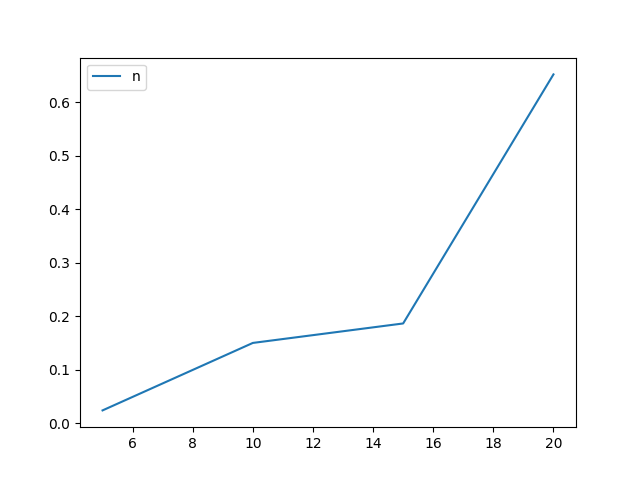
\includegraphics[scale=0.8]{imgs/2.2.png}}
\end{figure*}

Nous observons que le temps d'optimisation moyenne augmente très rapidement quand n et p devient grand. En effet le nombre de variable et de contrainte sont dépendente de n et de p, au plus ils sont grand au plus on a des variables et des contraintes et du coup nous mettons plus temps pour faire l'optimisation.


\newpage
\section{Application a la selection multicritere de projets}
\subsection{}

\begin{align*}
    \max f(x) =  \sum_{i}^n w_iz_i \\
    = \max \sum_{k=1}^n w'_k(kr_k- \sum_{i=1}^n b_{ik})
\end{align*}

\begin{center}
$ s.c.  \begin{cases}
r_k - b_{ik} \leq z_i(x) , i = 1,\cdots,n\\
\sum_{j = 1}^p x_{j}c_j \leq b\\
        \end{cases} $
\end{center}
$$ r_{k}, b_{ik} \geq 0 ; i\in \{1,\cdots, n\} ; j \in \{1,\cdots,p\} ; x_{j} \in \{0,1\}\\$$
avec $z_i(x) = \sum_{j=1}^p u_{ij}x_{j}$ et $ b = 1/2 \sum_{k=1}^p c_k $\\

traduisons le formule pour répondre au question en prenant  $p=4; n=2$ et la matrice a = $[[19,6,17,2], [2,11,4,18]]$, cout = $[40,50, 60,50]$ et $w' = (1,1)$ trouver à partir de $w = (2,1)$. Ces valeurs sont issus du document optimequi20.pdf\\
\begin{align*}
& \max\sum_{k=1}^2w'_k(kr_k-\sum_{i=1}^2b_{ik}) \\
& = (r_1-(b_{11}+b_{21}))+(2r_2-(b_{12}+b_{22}))\\
\end{align*}

\begin{center}
$ s.c.  \begin{cases}
r_1 - b_{11} \leq z_1(x) = 19x_{1} + 6x_{2} + 17x_{3}+ 2x_{4} \\
r_1 - b_{21} \leq z_2(x)  = 2x_{1} + 11x_{2} + 4x_{3}+ 18x_{4}\\
r_2 - b_{12} \leq z_1(x) = 19x_{1} + 6x_{2} + 17x_{3}+ 2x_{4}\\
r_2 - b_{22} \leq z_2(x) = 2x_{1} + 11x_{2} + 4x_{3}+ 18x_{4}\\
\sum_{j = 1}^4 x_{j}c_j \leq b = 100\\
        \end{cases} $\\
\end{center}
$\iff$
\begin{center}
$ s.c.  \begin{cases}
r_1 - b_{11} - 19x_{1} - 6x_{2} - 17x_{3}- 2x_{4} \leq  0 \\
r_1 - b_{21} - 2x_{1} - 11x_{2} -  4x_{3}- 18x_{4}\leq 0\\
r_2 - b_{12} - 19x_{1} - 6x_{2} - 17x_{3}- 2x_{4} \leq 0 \\
r_2 - b_{22} - 2x_{1} - 11x_{2} -  4x_{3}- 18x_{4} \leq 0\\
40x_1 + 50x_2 + 60x_3+50x_4 \leq 100\\
        \end{cases} $\\
\end{center}\\
$$ r_{k}, b_{ik} \geq 0 ; i\in \{1,\cdots, n\} ; j \in \{1,\cdots,p\} ; x_{j} \in \{0,1\}$$\\

En mettant le PL ci-desssus dans gurobi, nous trouvons comme solution optimale : 
\begin{align*}
& x_1 = 1.0;
x_2 = 0.0;
x_3 = 0.0;
x_4 = 1.0\\ 
& b_{11} = 0; 
b_{12} = 0 ;
b_{21} = 0 ;
b_{22} = 1\\
& (z_1, z_2) = (21, 20)\\
\end{align*}
\begin{center}
    le max de fonction objectif est de 61\\
    la satisfaction moyenne est de $(z_1(x) + z_2(x)) /2 = 20.5$
\end{center}\\

ensuite pour $w = (10 ,1)$ nous avons $w' = (9,1)$ changeons le fonction objectif : 
$$ 9(r_1-(b_{11}+b_{21}))+(2r_2-(b_{12}+b_{22}))$$
    





\pagebreak
\section{Application a la recherche d’un chemin robuste dans un graphe}
\subsection{}




soit $x_{ij}$ les variables boolean binaire tel que  $x_{ij}\in \{0 ,1\}$ et $i, j \in G$ avec $G = \{a,b,c,d,e,f,g\}$, $x_{ij}$ representant un arc allant de sommet i a la sommet j. $t_{ij}$ represente le temps necessaire pour aller du sommet i vers sommet j.

de maniere generale le PL de plus court chemin est : 
\begin{align*}
    \min \sum_{i,j \in G} x_{ij}t_{ij}^s \\
    s.c.\begin{cases}
            \sum_j x_{ij} - \sum_j x_{ji} = 0 
        \end{cases}\\
\end{align*}
$$x_{ij} \in (0,1), t_{ij}^s \in N$$ 

En adapdant le PL au graph G  on a  :
\begin{align*}
    \min \sum_{i,j \in G} x_{ij}t_{ij}^s \\
\end{align*}

\begin{align*}
        s.c.\begin{cases}
            x_{ab} + x_{ac} + x_{ad} = 1\\
            x_{bd} + x_{bc} + x_{be} = x_{ab}\\
            x_{ce} + x_{cf} = x_{ac} + x_{bc} + x_{dc}\\
            x_{dc} + x_{df} = x_{ad} + x_{bd}\\
            x_{eg} = x_{be} + x_{ce}\\
            x_{fg} = x_{cf} + x_{df}\\
        \end{cases}\\
\end{align*}

$$x_{ij} \in (0,1), t_{ij}^s \in N$$ 

\subsection{}
\begin{align*}
    \max f(x) =  \sum_{i}^n w_iz_i\\
     = \max \sum_{k=1}^n w'_k(kr_k- \sum_{i=1}^n b_{ik})
\end{align*}
\begin{align*}
       s.c.\begin{cases}
        r_k - b_{ik} \leq z_i(x) , i = 1,\cdots,n\\
        \sum_j x_{ij} - \sum_j x_{ji} = 0
        \end{cases}\\
\end{align*}\\
avec $z_{i} = \sum_{(i,j) \in P } t_{ij}^s =  \sum_{(i,j) \in G} x_{ij}t_{ij}^s$\\

reecrivons ce PL pour repondre au question avec $w' = (1,1)$ (trouver a partir de $w = (2,1)$, $n =2$  : 
\begin{align*}
    & \max \sum_{k=1}^2 w'_k(kr_k- \sum_{i=1}^2 b_{ik})\\
    & = w'_1(r_1 - (b_{11} - b_{21})) + w'_2(2r_k - (b_{12} + b_{22})) \\
    & = (r_1 - (b_{11} - b_{21})) + (2r_k - (b_{12} + b_{22})) \\
\end{align*}
\begin{align*}
       s.c.\begin{cases}
        r_1 - b_{11} \leq -z_1(x)\\
        r_1 - b_{21} \leq -z_2(x) \\
        r_2 - b_{12} \leq -z_1(x) \\
        r_2 - b_{22} \leq -z_2(x) \\
        x_{ab} + x_{ac} + x_{ad} = 1\\
        x_{bd} + x_{bc} + x_{be} = x_{ab}\\
        x_{ce} + x_{cf} = x_{ac} + x_{bc} + x_{dc}\\
        x_{dc} + x_{df} = x_{ad} + x_{bd}\\
        x_{eg} = x_{be} + x_{ce}\\
        x_{fg} = x_{cf} + x_{df}\\
        \end{cases}\\
\end{align*}\\
avec $z_{1}(x) = 5x_{ab}+10x_{ac}+2x_{ad} + 4x_{bc} + x_{bd} + 4x_{be}  +  3x_{ce} + x_{cf} +  x_{dc} + 3x_{df} + x_{eg} + x_{fg}$\\
$z_2(x) = 3x_{ab}+ 4x_{ac}+6x_{ad} + 2x_{bc} + 3x_{bd} + 6x_{be}  +  x_{ce} + 2x_{cf} +  4x_{dc} + 5x_{df} + x_{eg} + x_{fg}$




\newpage
\end{justify}
\end{flushleft}
\end{document}

